\chapter{Methodology}
\label{chap:methodology}

\section{Research Design}

This thesis adopted a replication-and-extension design to evaluate whether a common \gls{xai} framework could be applied consistently across heterogeneous medical-prediction studies. The research comprised three connected stages. First, five published studies were reconstructed using their reported datasets, preprocessing decisions, model families, and evaluation procedures. Second, corrected analytical branches were introduced when literal reconstruction would cause information leakage or use held-out test data for model selection. Such practices can produce optimistically biased estimates of predictive performance \citep{collins_tripodai_2024, moons_probastai_2025}. Third, the resulting fitted models were passed to a common \gls{xai} pipeline that generated global explanations, local explanations, method-agreement measures, and explanation-stability estimates when retraining was available.

The study distinguishes among three analytical operations:

\begin{enumerate}
    \item \textbf{Replication}, referring to the reconstruction of the workflow described by each source study.
    \item \textbf{Methodological correction}, referring to changes introduced to preserve the separation of training and test information and prevent test-set-driven model selection.
    \item \textbf{\gls{xai} extension}, referring to the application of the standardised explanation framework to a fitted model derived from each study.
\end{enumerate}

Exact reconstruction of a published workflow does not necessarily produce a methodologically valid predictive evaluation when the reported procedure contains leakage or uses test data during model development \citep{collins_tripodai_2024, moons_probastai_2025}. When reconstruction and leakage-controlled evaluation differed, the paper-style result was retained and identified as such, while the corrected branch supplied the model and data used for the \gls{xai} extension. The study evaluates fitted models and their explanation artefacts within a computational model-audit setting. It does not assess clinical effectiveness, establish causal relationships, or propose the models for deployment in clinical practice.

\section{Literature Review and Study Selection}

The introduction, state-of-the-art review, and selection of studies for replication were informed by a structured literature search designed to identify relevant healthcare \gls{xai} research and replicable empirical studies. Searches covered IEEE Xplore, Google Scholar, PubMed Central, ScienceDirect, Springer Nature, Scopus, and the ACM Digital Library. Supplementary discovery sources, including ResearchGate, and reference-list exploration were used to identify additional relevant and frequently cited studies.

Screening was conducted in stages. Titles and abstracts were first examined to remove duplicate, non-clinical, non-predictive, or otherwise irrelevant records. Potentially eligible papers were then read in full and assessed according to their methodological relevance, availability of the underlying dataset, description of the analytical workflow, and suitability for computational replication. Recent, frequently cited, and strongly connected publications were prioritised during exploration, although citation frequency was not treated as evidence of methodological quality.

The search was conducted to support the state-of-the-art analysis and identify suitable studies for replication rather than to estimate a pooled clinical effect. Complete database-specific search strings, exact search dates, and record-level counts for every screening stage were not retained. The process is therefore reported as a structured literature search and study-selection procedure, not as a systematic review. No retrospective screening counts were constructed.

Five studies were selected because they collectively provided variation in clinical domain, sample size, feature dimensionality, model family, class imbalance, and analytical purpose. They addressed heart disease, stroke, diabetes mellitus, \gls{ckd}, and hospital readmission in relation to \gls{hbaone} measurement \citep{khanna_comparative_2015, wu_machine_2024, chang_pima_2023, santhiya_chronic_2024, strack_impact_2014}.


\section{Datasets and Final Analytical Configurations}

All datasets were obtained from publicly accessible repositories or from the source-study data package, and personally identifying fields were excluded from modelling. The final analytical configurations differed in model family, data partitioning, scoring metric, feature representation, and the availability of retraining. These characteristics are summarised in Table~\ref{tab:final-configurations} because they determine how each fitted model was supplied to the common \gls{xai} framework and which analyses could be performed.

\begin{table}[htbp]
    \centering
    \caption{Final analytical configurations supplied to the standardised \gls{xai} framework. Training and test counts refer to held-out partitions except for \gls{hbaone}, for which the complete eligible cohort was used as both reference and explanation data in accordance with its full-cohort inferential design.}
    \label{tab:final-configurations}
    \begin{tabular}{lrrrrl}
        \hline
        Dataset & Training & Test & Features & Outcome & \gls{xai} model \\
        \hline
        Heart disease & 148 & 149 & 13 & Binary & Logistic regression \\
        Stroke & 4,087 & 1,022 & 7 & Binary & Balanced logistic regression \\
        Diabetes & 538 & 230 & 5 & Binary & \Gls{rf} \\
        \gls{ckd} & 280 & 120 & 24 & Binary & \Gls{rf} \\
        \gls{hbaone}/readmission & 69,970 & 69,970 & 90\textsuperscript{a}
            & Binary & Statsmodels logistic model \\
        \multicolumn{6}{l}{\footnotesize
        \textsuperscript{a} Non-intercept explanatory terms; the complete
        Patsy design matrix contained 91 columns including the intercept.} \\
        \hline
    \end{tabular}
\end{table}

As shown in Table~\ref{tab:final-configurations}, \gls{hbaone} has identical reference and explanation counts. These counts do not represent a held-out predictive experiment. The source study used a full-cohort inferential logistic-regression design, so the complete eligible design matrix was supplied as both reference and explanation data to satisfy the common framework interface. The resulting \gls{hbaone} explanations are therefore interpreted as in-sample descriptions of the fitted statistical model rather than as estimates of predictive generalisation.

\subsection{Heart Disease}

The processed Cleveland heart-disease data were loaded from the local UCI-format file used by the replicated comparative study \citep{khanna_comparative_2015}. Missing values denoted by question marks were converted to missing values, incomplete observations were removed, and the original multi-level diagnostic outcome was converted to absence versus presence of heart disease. The cleaned sample contained 297 observations and 13 predictors.

An equal, stratified training/test partition was used to follow the source study. Standardisation parameters were estimated exclusively from the training partition and then applied to the test partition. Logistic regression with five-fold and ten-fold internal \gls{cv}, three \gls{svm} kernels, and the reported neural-network families were compared descriptively. Ten-fold L2-regularised logistic regression was pre-specified for the \gls{xai} extension because it represented a central replicated model and provided a probabilistic, coefficient-based baseline. Held-out performance rankings were not used to make this selection.

The four multi-level variables \texttt{cp}, \texttt{thal}, \texttt{slope}, and \texttt{restecg} were retained in their source-coded numeric form to preserve the 13-predictor representation used in the replicated study. This choice supports fidelity to the original analytical specification, but it also imposes a linear ordering on category codes within logistic regression. Coefficients and \gls{lime} intervals involving these variables are therefore interpreted as behaviour of the reproduced coded model rather than as evidence that the clinical categories form an ordered scale. One-hot encoding and alternative contrast specifications remain appropriate sensitivity analyses for future work.

\subsection{Stroke}

The stroke dataset was restricted to valid binary gender categories, and the identifier field was removed before reconstructing the published stroke-prediction comparison \citep{wu_machine_2024}. A missingness indicator was created for \gls{bmi}. The data were split using a stratified 80:20 partition before any learned preprocessing operation. Mean \gls{bmi} imputation was estimated from the training partition, categorical dummy columns were derived from the training categories and aligned in the test data, and standardisation was fitted on training data only.

The reduced feature set was identified using absolute correlations with the outcome greater than 0.1, calculated only within the training partition. This produced seven predictors in the final extension. The paper-style comparison of logistic regression, \gls{dt}, \gls{rf}, \gls{svm}, \gls{knn}, XGBoost, and a \gls{dnn} was retained. A class-balanced logistic-regression model was pre-specified for \gls{xai} to address the severe class imbalance and to provide a stable probabilistic baseline. The held-out model comparison remained descriptive.

\subsection{Diabetes}

The Pima Indians Diabetes dataset contained 768 observations and eight predictors, following the study by \citet{chang_pima_2023}. Zero values in glucose, blood pressure, skin thickness, insulin, and \gls{bmi} were treated as physiologically invalid missing values. Descriptive \gls{pca} and clustering analyses were retained as exploratory full-dataset analyses and were not used to estimate predictive performance.

For predictive modelling, the stratified split was performed before median imputation. Medians were estimated from the 538 training observations and applied unchanged to the 230 test observations. \Gls{dt}, \gls{rf}, and Gaussian naive Bayes models were evaluated using the complete predictor set and the three- and five-feature configurations defined by the source study. A \gls{rf} using the five-feature configuration was pre-specified for the \gls{xai} extension. This choice preserved the source-defined reduced feature set and enabled comparison of native tree importance, permutation importance, and \gls{shap} importance; it was not selected by maximising test accuracy.

\subsection{Chronic Kidney Disease}

The \gls{ckd} dataset contained 400 observations and was analysed using the classifier families reported by \citet{santhiya_chronic_2024}. Formatting artefacts and malformed missing-value markers were harmonised, the identifier was removed, and the outcome was encoded as \gls{ckd} versus non-\gls{ckd}. The source-study workflow - random-sample imputation and label encoding before a 70:30 split - was retained in an explicitly labelled paper-style branch so that its reported behaviour could be examined.

A second branch controlled information leakage by splitting first. Missing values in both training and test data were sampled only from the observed training distribution, with training-derived mean or mode values used as fallbacks. Categorical encoding was fitted on training data, with unseen test categories assigned a reserved value. The same \gls{knn}, \gls{dt}, \gls{rf}, naive-Bayes, and gradient-boosting families were evaluated in both branches. The corrected branch supplied the \gls{xai} data and model. \Gls{rf} was pre-specified because it was the leading classifier reported by the source study, not because it ranked first on the present test partition.

Row-level integrity checks found 400 unique identifiers, no exact duplicate predictor--outcome rows after removal of the identifier, and no identical predictor profile shared between the stratified training and test partitions. Repeating the comparison after training-fitted imputation and encoding likewise found no exact duplicates within either partition and no exact cross-partition profile overlap. The near-perfect held-out results were therefore not explained by exact duplicated records, although the dataset remains small and produced an unusually separable internal evaluation.

\subsection{\gls{hbaone} and Hospital Readmission}

The \gls{hbaone} analysis reconstructed the cohort and inferential design reported by \citet{strack_impact_2014}. The outcome indicated readmission within 30 days. Variables excluded by the source study were removed, missing race and medical-specialty categories were represented explicitly, coded admission and discharge fields were mapped to readable groups, and only the first encounter for each patient was retained. Encounters with invalid gender coding or discharge dispositions associated with death or hospice were excluded.

The analysis reconstructed the four-level \gls{hbaone} variable and grouped demographic, admission, discharge, specialty, age, and primary-diagnosis covariates. Nested logistic-regression specifications were fitted with Statsmodels, culminating in an interaction-rich model containing \gls{hbaone}-by-diagnosis and selected clinical-context interactions. The final Patsy design matrix contained 91 columns for 69,970 eligible encounters, comprising one intercept and 90 non-intercept explanatory terms. The intercept was excluded from feature-importance comparisons.

This analysis estimates conditional associations within the observed cohort and is not directly equivalent to the four held-out prediction studies. Coefficients and odds ratios retain their inferential interpretation, whereas the \gls{xai} outputs describe behaviour of the fitted model. No causal effect of \gls{hbaone} testing or medication change is inferred from the explanations.

\section{Predictive Validation and Uncertainty}

Heart disease, stroke, diabetes, and \gls{ckd} were evaluated on their respective held-out test partitions. \gls{hbaone} was excluded from this comparison because its source design fitted an inferential model to the complete eligible cohort. Predicted probabilities were converted to binary classes using a prespecified threshold of 0.5 \citep{hernandez-orallo_unified_2012}. This fixed threshold was used consistently for computational evaluation and was not selected as a clinical decision threshold.

For binary outcomes, accuracy, precision, recall, specificity, and the F1 score were calculated from the confusion matrix as follows \citep{powers_evaluation_2011}:

\begin{align}
\mathrm{Accuracy}
    &= \frac{TP+TN}{TP+TN+FP+FN}, \\
\mathrm{Precision}
    &= \frac{TP}{TP+FP}, \\
\mathrm{Recall}
    &= \frac{TP}{TP+FN}, \\
\mathrm{Specificity}
    &= \frac{TN}{TN+FP}, \\
F_1
    &= 2\frac{\mathrm{Precision}\times\mathrm{Recall}}
    {\mathrm{Precision}+\mathrm{Recall}}.
\end{align}

Here, \gls{tp}, \gls{tn}, \gls{fp}, and \gls{fn} are the four confusion-matrix outcomes. \gls{rocauc} was interpreted as the probability that the fitted model assigns a higher score to a randomly selected positive observation than to a randomly selected negative observation, with half credit assigned to tied scores \citep{fawcett_introduction_2006}:

\begin{equation}
\mathrm{ROC\ AUC}
=
P\left(s(X^{+}) > s(X^{-})\right)
+
\frac{1}{2}
P\left(s(X^{+}) = s(X^{-})\right),
\end{equation}

where $s(\cdot)$ denotes the model prediction score. Average precision was used to summarise the precision-recall curve, which is particularly informative when the outcome classes are imbalanced \citep{saito_precision-recall_2015}.

Uncertainty in the held-out metrics was estimated using a non-parametric observation-level bootstrap \citep{efron_introduction_1993}. In each bootstrap repetition, the observed labels and corresponding predicted probabilities were sampled together with replacement, while the fitted model remained fixed. For metric $M$, its value in bootstrap repetition $b$ was calculated as

\begin{equation}
M^{*(b)}
=
M\left(
\left\{y_{i_r},\widehat{p}_{i_r}\right\}_{r=1}^{n}
\right),
\qquad b=1,\ldots,B,
\end{equation}

where the indices $i_1,\ldots,i_n$ were sampled with replacement from the held-out observations. The analysis used $B=5000$ bootstrap resamples and random seed 42. Following the percentile method, the 95\% bootstrap confidence interval was calculated as \citep{efron_introduction_1993}

\begin{equation}
\mathrm{CI}_{95\%}
=
\left[
Q_{0.025}\left(M^*\right),
Q_{0.975}\left(M^*\right)
\right].
\end{equation}

These intervals quantify uncertainty associated with the held-out observations for the fixed model predictions. They do not incorporate uncertainty from model selection, model retraining, or population shift.


\section{Standardised \gls{xai} Framework}

Each replication notebook supplied a fitted binary model, aligned reference and explanation matrices, binary labels, ordered feature names, a scoring rule, an output directory, and a retraining callback where available. A common experiment runner then applied the same global, local, stability, metadata, and export stages. Global permutation importance used \gls{rocauc} in all five configurations. This common continuous scorer avoided the coarse increments and tied zero values that accuracy can produce on small test sets, while retaining discrimination as the quantity evaluated across datasets. Bootstrap-refit stability used negative log loss, as described below, because that analysis assessed variation in predicted probabilities across refitted models.


\subsection{Architecture and Execution Flow}

The framework separates dataset-specific model development from shared explanation logic. The replication notebooks remain responsible for data loading, preprocessing, analytical correction, feature construction, model selection, and fitting. The shared framework begins only after a final fitted model and aligned matrices have been produced. This boundary prevents the explanation code from silently changing the analytical workflow that it is intended to audit.

Figure~\ref{fig:xai-framework-architecture} presents the execution architecture. A configuration dictionary initialises an \texttt{ExperimentState} containing the fitted model, matrices, labels, ordered feature names, and analysis settings. The \texttt{run\_pipeline} entry point creates an \texttt{XAIExperiment}, executes the global and local branches, invokes bootstrap-refit stability when a retraining callback is available, constructs provenance metadata, and exports the resulting artefacts. The three explanation branches share the same aligned inputs but answer different questions: the global branch compares feature-importance definitions for the fitted model, the local branch examines selected prediction outcomes and \gls{lime} seed sensitivity, and the stability branch evaluates ranking persistence after changes in training-sample composition.

\begin{figure}[htbp]
    \centering
    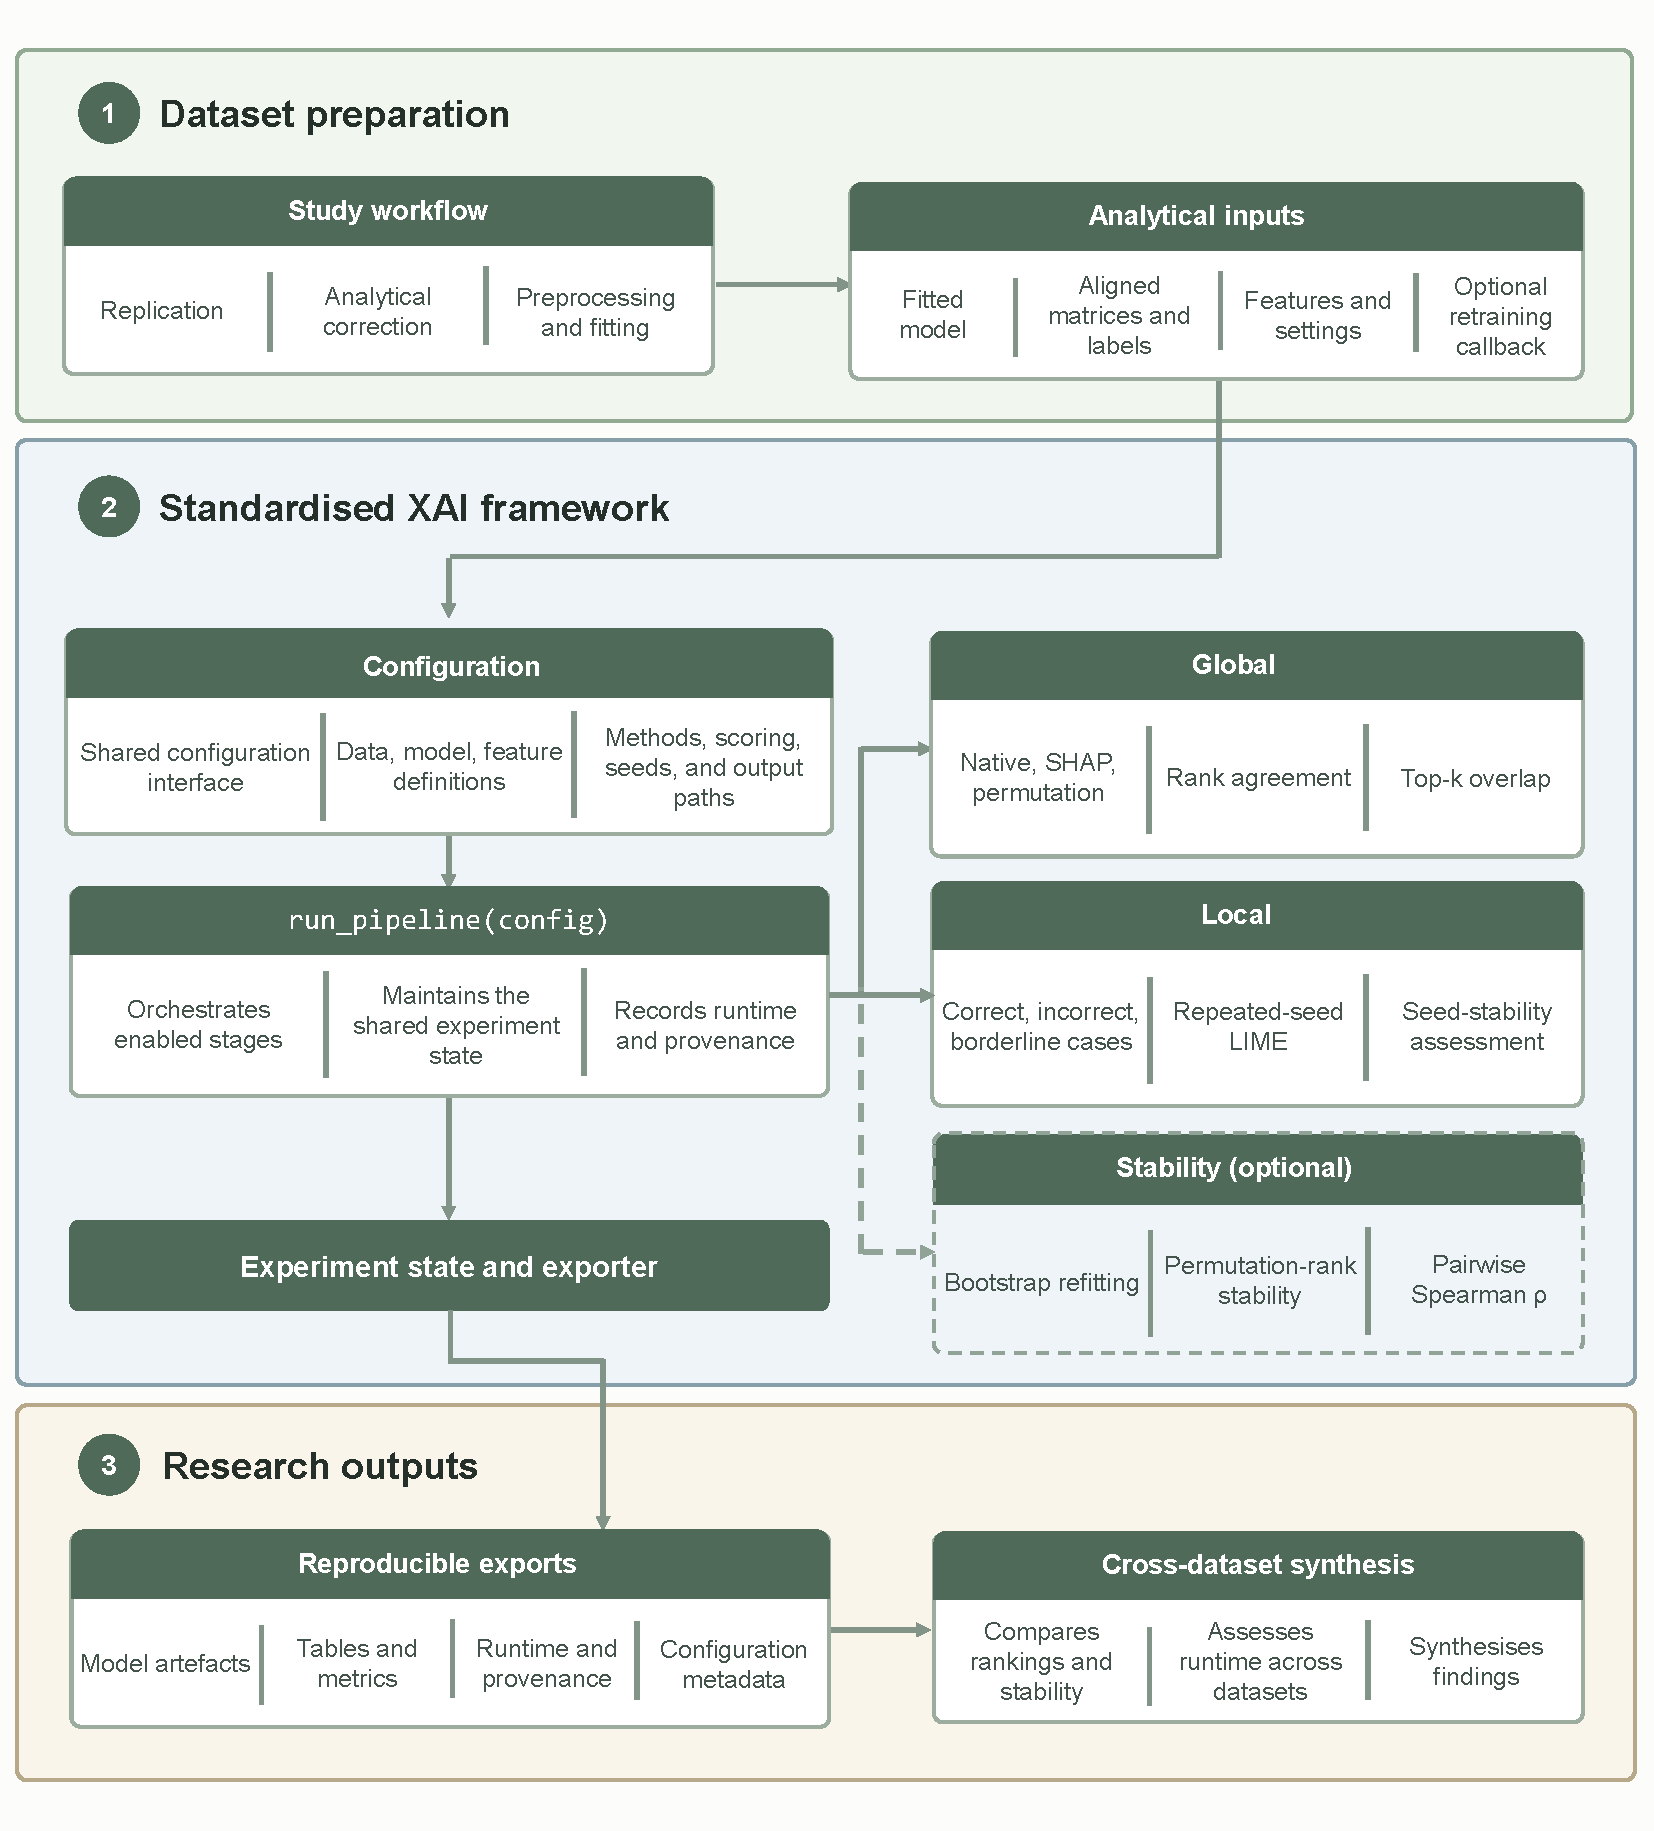
\includegraphics[width=\textwidth]{images/framework_architecture_portrait.pdf}
    \caption{Pipeline architecture for the standardised explainability and stability analysis. Dataset-specific notebooks prepare the fitted model and aligned inputs; the common runner executes the global and local explanation branches and exports reproducible outputs. The dashed border indicates the optional bootstrap-refit stability module, which requires a compatible model-retraining callback.}
    \label{fig:xai-framework-architecture}
\end{figure}

The framework stores intermediate and final outputs in the experiment state rather than returning unrelated method-specific objects. Global results contain native, permutation, and \gls{shap} importance tables together with rank comparisons. Local results contain the selected observations, all seed-specific \gls{lime} rules, aggregated rule summaries, and seed-stability measures. When enabled, the stability branch retains both bootstrap-level rankings and their summaries. The exporter then writes aligned \gls{csv} and \gls{json} files, the fitted model bundle, runtime versions, configuration metadata, and stage-level execution times. These outputs supply the later cross-dataset analysis without requiring access to the active notebook state.

\subsection{Configuration and Example Usage}

The public notebook interface is a single configuration dictionary passed to \texttt{run\_pipeline}. The required fields identify the dataset, fitted model, aligned training and explanation matrices, labels, and ordered feature names. Optional fields control permutation scoring, representative-case sampling, \gls{lime} repetitions, bootstrap-refit stability, and the output location. A retraining callback must accept one bootstrap training sample and return a newly fitted model with the same specification.

The following abbreviated Stroke example shows the interface after the repository package has been installed:

\begin{samepage}
\begin{small}
\begin{verbatim}
from xai_framework.run_pipeline import run_pipeline

config = {
    "dataset_name": "stroke",
    "model": final_model,
    "X_train": X_train_sel,
    "X_test": X_test_sel,
    "y_train": y_train,
    "y_test": y_test,
    "feature_names": list(X_train_sel.columns),
    "scoring": "roc_auc",
    "local_cases_per_type": 10,
    "lime_seeds": list(range(20)),
    "train_model_fn": train_model_fn,
    "stability_n_bootstrap": 100,
    "stability_scoring": "neg_log_loss",
    "output_dir": "../../results/stroke",
}

experiment = run_pipeline(config)
\end{verbatim}
\end{small}
\end{samepage}

The call executes the enabled stages sequentially and exports their outputs to the configured directory. The returned \texttt{experiment} object also retains the same results in memory for notebook inspection. If \texttt{train\_model\_fn} is omitted, global and local explanations are still generated, while bootstrap-refit stability is recorded as unavailable. This behaviour allowed the same interface to accommodate the four held-out predictive configurations and the \gls{hbaone} inferential configuration without substituting a non-equivalent retraining procedure.

\subsection{Global Explanations}

Three global importance representations were generated where supported:

\begin{itemize}
    \item \textbf{Native importance}: absolute model coefficients for linear models, absolute non-intercept parameters for the Statsmodels model, or impurity-based feature importance for tree ensembles. Signed coefficient and parameter values were retained separately where available \citep{breiman_random_2001, linardatos_explainable_2020}.

    \item \textbf{Permutation importance}: decrease in the configured score after feature permutation, calculated using 20 repetitions and a fixed random seed of 42. The mean and standard deviation across permutations were exported \citep{fisher_models_2019}.

    \item \textbf{\gls{shap} importance}: mean absolute \gls{shap} value for global attribution magnitude and mean signed \gls{shap} value for average attribution direction \citep{NIPS2017_8a20a862}. The explainer used for each final configuration is reported in Table~\ref{tab:shap-explainers}. Tree models used the tree-specific algorithm. For the remaining models, the fitted prediction function and reference matrix were supplied to \gls{shap}'s automatic interface; \gls{shap}~0.51.0 selected exact enumeration when this was computationally feasible and permutation-based approximation otherwise.
\end{itemize}

\begin{table}[htbp]
    \centering
    \caption{\gls{shap} explainer used for each final analytical configuration. The class names report the algorithms instantiated by \gls{shap}~0.51.0, rather than inferring an explainer solely from the model family.}
    \label{tab:shap-explainers}
    \begin{tabular}{lll}
        \toprule
        Dataset & Model supplied to the framework & \gls{shap} explainer \\
        \midrule
        Heart disease & Logistic regression & PermutationExplainer \\
        Stroke & Logistic regression & ExactExplainer \\
        Diabetes & \Gls{rf} & TreeExplainer \\
        \gls{ckd} & \Gls{rf} & TreeExplainer \\
        \gls{hbaone}/readmission & Statsmodels logistic model & PermutationExplainer \\
        \bottomrule
    \end{tabular}
\end{table}

The Heart and Stroke models were linear, but the framework supplied their probability-prediction functions to the generic \gls{shap} interface rather than passing the estimator directly to \texttt{LinearExplainer}. Consequently, the resulting classes were \texttt{PermutationExplainer} for the 13-feature Heart model and \texttt{ExactExplainer} for the seven-feature Stroke model. The 91-column \gls{hbaone} design matrix likewise required \texttt{PermutationExplainer}. These model-agnostic explainers describe the supplied prediction functions relative to their reference matrices; they should not be reported as \texttt{LinearExplainer} or \texttt{KernelExplainer} results.

For linear models, native global importance was operationally defined using the absolute coefficient magnitude \citep{linardatos_explainable_2020}:

\begin{equation}
I_j^{\mathrm{native}}
=
\left|\beta_j\right|,
\end{equation}

where $\beta_j$ is the fitted coefficient associated with feature or design-matrix term $j$. For tree ensembles, the estimator's impurity-based feature importance was used \citep{breiman_random_2001}.

Permutation importance for feature $j$ was calculated as the decrease in the configured score after permutation \citep{fisher_models_2019}:

\begin{equation}
I_j^{\mathrm{perm}}
=
S(f,X,y)
-
\frac{1}{N_{\mathrm{perm}}}
\sum_{r=1}^{N_{\mathrm{perm}}}
S\left(f,X_{\pi_j}^{(r)},y\right),
\end{equation}

where $N_{\mathrm{perm}}=20$ is the number of permutation repetitions, $S$ is \gls{rocauc} for the global fitted-model analyses, $f$ is the fixed fitted model, and $X_{\pi_j}^{(r)}$ denotes the data in repetition $r$ after feature $j$ has been permuted.

Global \gls{shap} importance for feature $j$ was calculated as its mean absolute attribution across the explanation observations \citep{NIPS2017_8a20a862}:

\begin{equation}
I_j^{\mathrm{SHAP}}
=
\frac{1}{n}
\sum_{i=1}^{n}
\left|\phi_{ij}\right|,
\end{equation}

where $\phi_{ij}$ is the \gls{shap} value assigned to feature $j$ for observation $i$, and $n$ is the number of observations in the explanation matrix.

Importance magnitudes were not compared directly across methods because native, permutation, and \gls{shap} importance have different definitions, scales, and interpretations \citep{linardatos_explainable_2020, vilone_classification_2021}. Features were instead ranked within each method, with average ranks assigned to tied values.

Agreement between methods $a$ and $b$ was quantified using Spearman rank correlation \citep{spearman_proof_1904}:

\begin{equation}
\rho_s^{(a,b)}
=
\operatorname{corr}
\left(
\mathcal{R}\left(I^{(a)}\right),
\mathcal{R}\left(I^{(b)}\right)
\right),
\end{equation}

where $\mathcal{R}(\cdot)$ converts the aligned feature-importance values into ranks. This correlation-of-ranks formulation accommodates the average ranks assigned to tied values. Agreement was calculated using features available in both methods. When native importance was unavailable, the comparison was restricted to \gls{shap} and permutation importance.

\subsection{Representative Cases and \gls{lime}}

Local explanations were generated for five representative case types: true positive, true negative, false positive, false negative, and borderline. Using the prespecified classification threshold of 0.5 \citep{hernandez-orallo_unified_2012}, up to ten observations were selected for each available type. True positives and false positives were ordered by decreasing predicted probability, while true negatives and false negatives were ordered by increasing predicted probability. After these four outcome groups had been selected, up to ten additional observations closest to the threshold were assigned to the borderline group. This ordering prevented the same observation from appearing under two case labels. A group contained fewer than ten observations when the corresponding outcome was rare and was omitted when no such observation existed.

For an observation $x$, \gls{lime} estimates an interpretable local surrogate according to \citet{ribeiro_why_2016}:

\begin{equation}
\xi(x)
=
\arg\min_{g\in G}
\left[
\mathcal{L}\left(f,g,\pi_x\right)
+
\Omega(g)
\right],
\end{equation}

where $f$ is the fitted prediction model, $g$ is an interpretable local surrogate, $\pi_x$ weights perturbed observations according to their proximity to $x$, $\mathcal{L}$ measures local disagreement between $f$ and $g$, and $\Omega(g)$ penalises surrogate complexity.

\gls{lime} was fitted using the corresponding training matrix as its reference distribution. Each selected observation was explained under 20 perturbation seeds, numbered 0--19, and five rules were retained from each fitted local surrogate. Raw outputs preserved the case identifier, case type, seed, rule rank, signed weight, predicted class, and predicted probability. For each observation and rule, weights were averaged across seeds and their standard deviation was retained. Category-level summaries additionally reported the number of cases and seeds contributing to each rule, its selection frequency, mean absolute weight, median signed weight, and the proportion of positive weights.

Seed sensitivity was quantified separately for each observation. The analysis calculated the mean pairwise Spearman correlation between the 20 seed-specific rule rankings, mean overlap among the three strongest absolute-weight rules, mean rule-weight standard deviation, and mean sign consistency. The illustrative figures retained the highest-ranked observation in each case category and displayed weights averaged over the 20 seeds; the broader RQ3 summaries used all selected observations. For the positive-class explanation, positive \gls{lime} weights indicate movement towards the positive class, while negative weights indicate movement away from it \citep{ribeiro_why_2016}. These weights describe fitted local surrogates and are not equivalent to global feature effects, regression coefficients, or causal effects \citep{ribeiro_why_2016, vilone_classification_2021}.

\subsection{Explanation Stability}

Stability analysis was performed only for datasets whose replication notebook supplied a retraining callback. For each eligible dataset, 100 stratified bootstrap samples were drawn with replacement from the final aligned training matrix. Sampling was performed within outcome classes so that every bootstrap sample retained the original class counts, while individual observations could appear more than once or be omitted. A new model with the same specification and fixed model seed was fitted to each bootstrap sample.

Permutation importance was calculated for every refitted model on the unchanged held-out test partition using negative log loss, ten permutation repetitions, and a fixed permutation seed \citep{fisher_models_2019}. Using the same probability-based scorer for Heart, Stroke, Diabetes, and \gls{ckd} avoided the coarse increments and tied zero values produced by accuracy on small test sets. Feature-level summaries reported the mean and standard deviation of importance and rank, together with the frequency with which each feature appeared among the three highest-ranked features.

The canonical \gls{hbaone} bundle did not supply a validated retraining callback, so no result from that configuration was included in the principal stability comparison. An exploratory sensitivity experiment separately reconstructed the Statsmodels fitting procedure for bootstrap samples and permuted groups of Patsy design columns corresponding to the same original variable. One hundred refits were requested, but only 58 converged. Because analysing only the successful refits could introduce selection bias if convergence depended on the sampled observations, the experiment was used to assess computational feasibility and was not incorporated into the principal cross-dataset stability comparison.

For $K$ bootstrap refits, mean pairwise rank stability was defined as

\begin{equation}
\overline{\rho}
=
\frac{2}{K(K-1)}
\sum_{a<b}
\operatorname{corr}
\left(
\mathcal{R}\left(I^{(a)}\right),
\mathcal{R}\left(I^{(b)}\right)
\right),
\end{equation}

where $I^{(a)}$ is the aligned vector of permutation-importance values from bootstrap refit $a$, and $\mathcal{R}(\cdot)$ converts importance values into ranks. Average ranks were assigned to tied values. Spearman correlation therefore evaluates whether the relative ordering of features persists when the composition of the training sample changes \citep{spearman_proof_1904}.

Mean top-three overlap was calculated as

\begin{equation}
\overline{O}_3
=
\frac{2}{K(K-1)}
\sum_{a<b}
\frac{
\left|T_3^{(a)}\cap T_3^{(b)}\right|
}{3},
\end{equation}

where $T_3^{(a)}$ contains the three highest-ranked features from bootstrap refit $a$. Pairwise overlap ranges from 0, when two top-three sets share no features, to 1, when they are identical. With $K=100$ refits, each reported mean summarised 4,950 pairwise comparisons.

This design measures sensitivity to variation in the composition of the final training matrix. The held-out test set, model seed, permutation seed, scoring rule, and number of permutation repetitions remained fixed. It is not repeated \gls{cv} and does not assess alternative train--test partitions, preprocessing uncertainty before construction of the final aligned matrix, \gls{shap} background selection, or repeated \gls{lime} perturbations \citep{lofstrom_meta_2022, canha_functionally-grounded_2025}.

\section{Cross-Dataset Analysis}

The exported dataset-level results were analysed in a separate cross-dataset notebook. Global agreement was summarised using the within-dataset Spearman correlations described previously. For methods $a$ and $b$, top-$k$ overlap was defined as

\begin{equation}
O_k^{(a,b)}
=
\frac{
\left|T_k^{(a)}\cap T_k^{(b)}\right|
}{k},
\end{equation}

where $T_k^{(a)}$ and $T_k^{(b)}$ are the sets of the $k$ highest-ranked features under methods $a$ and $b$, respectively. The cross-dataset analysis used $k=5$. The resulting value ranges from 0, when the two sets contain no common features, to 1, when the sets are identical. This measure represents the proportion of shared top-ranked features and is distinct from the Jaccard coefficient, whose denominator is the size of the union. Top-feature overlap complements rank correlation by assessing agreement among the most highly ranked features \citep{lofstrom_meta_2022, canha_functionally-grounded_2025}.

For visualisation, importance values were normalised independently within each method and dataset:

\begin{equation}
\widetilde{I}_{j,m}
=
\frac{I_{j,m}}
{\max_{\ell} I_{\ell,m}},
\end{equation}

where $I_{j,m}$ is the importance of feature $j$ under method $m$, and the denominator is the largest importance observed under that method for the same dataset. This transformation rescales each value relative to the largest within-method importance. It does not place native, permutation, and \gls{shap} importance on a common inferential scale. Negative permutation values were retained in both the exported results and the visualisations. These values indicate that permuting the feature increased the observed score in that evaluation sample and do not represent negative clinical effects \citep{fisher_models_2019}.

Local explanations were compared according to representative case type, prediction correctness, and mean absolute \gls{lime} weight. Global-local feature presence was operationalised as the occurrence of globally high-ranked feature names within the strongest \gls{lime} rule strings. This lexical measure records whether the same feature names occur in the global and local outputs. It does not measure agreement in attribution sign, magnitude, rule interval, or local-surrogate fidelity \citep{ribeiro_why_2016, vilone_classification_2021}.

The cross-dataset synthesis was descriptive because the datasets differ in their populations, outcomes, feature definitions, sample sizes, preprocessing procedures, and model families. Similarly named variables from different datasets were not assumed to be clinically or statistically interchangeable \citep{moons_probastai_2025}. \gls{hbaone} was interpreted separately as an in-sample inferential-model case when considering explanation stability and generalisability.

\section{Reproducibility and Verification}

The final implementation ran on Windows using CPython 3.12.6 and included exact focused and archival dependency locks. Each canonical experiment exported the aligned data, labels, ordered feature names, fitted model, metadata, and \gls{xai} tables. Runtime metadata recorded the Python version, platform, and relevant library versions. A package-level command-line interface allowed trusted saved bundles to be validated and rerun without overwriting the canonical notebook results.

Automated tests covered task detection, binary metrics, representative-case selection, native importance, ranking and tie handling, export round trips, command-line validation, safe output paths, bundle orchestration, result comparison, runtime provenance, bootstrap-refit stability, canonical scorer configuration, CKD record integrity, and a small end-to-end \gls{shap} and \gls{lime} integration pipeline. Statement coverage was measured with Coverage.py~7.11.0 over \texttt{src/xai\_framework}, including the real integration test. At final verification, all 62 tests passed in 73.52 seconds and 591 of 719 executable statements were covered, corresponding to 82\% statement coverage. All five canonical bundles also passed \gls{csv} and \gls{json} validation. Coverage quantifies which implementation statements were exercised by the tests; it does not assess statistical correctness or compatibility beyond the tested configurations.

Execution time was measured using Python's monotonic high-resolution timer. The framework recorded the global-explanation, local-explanation, optional stability, export, and total durations in \texttt{execution\_times.json} and copied the same record into each bundle's metadata. For a comparable timing experiment, the five trusted saved bundles were rerun once on the same Windows~11 workstation with an AMD Ryzen~7 3700U processor under CPython~3.12.6. These reruns used the aligned saved matrices, the fitted saved models, up to ten cases per available category, and 20 \gls{lime} seeds per case. They excluded model fitting and bootstrap-refit stability because a serialised fitted bundle does not contain the retraining callback. Background workload was not experimentally controlled. The timings are therefore descriptive single-run measurements of one execution environment rather than hardware-independent performance guarantees.

\section{Ethical and Methodological Scope}

The study used secondary research datasets and did not interact with patients or alter clinical care. Personally identifying fields were excluded from modelling, and no attempt was made to reidentify individuals. Public availability does not remove potential limitations arising from bias, under-representation, measurement error, missing data, historical clinical practices, or the construction of outcome labels. These factors can affect both predictive performance and the explanations derived from a fitted model \citep{moons_probastai_2025}. The reported results are therefore specific to the analysed datasets, preprocessing decisions, fitted models, and explanation configurations.

\gls{shap}, \gls{lime}, native importance, and permutation importance describe relationships learned or used by fitted models according to different method-specific definitions. Their outputs do not establish that a feature causes an outcome or that an explanation is clinically correct \citep{vilone_classification_2021, tjoa_survey_2021}. The framework is evaluated as a reproducible computational instrument for auditing models and comparing explanation behaviour. Clinical actionability, safety, fairness, and appropriate use would require additional evidence involving relevant patient groups, healthcare professionals, clinical workflows, and prospective evaluation \citep{panigutti_co-design_2023, vasey_decideai_2022}. No subgroup fairness audit or clinical-utility evaluation was conducted in this dissertation.
